%% ------------------------------------------------------------------------- %%n
\chapter{Aprendizado Ativo}
\label{cap:aprendizado_ativo}

Nesse capítulo serão apresentados os fundamentos de aprendizado ativo. É importante citar que muitos dos trabalhos clássicos citados foram descobertos, principalmente, pela revisão da literatura de [\cite{settles2012active, settles2014active}]. Alguns outros trabalhos são também muito importantes nessa discussão, como os de [\cite{olsson2009literature}], focada em Linguagem Natural, o de [\cite{aggarwal2014active}\ e de [\cite{wang2011active}]. A própria revisão de literatura de [\cite{zhu2006semi}] também explica alguns conceitos fundamentais e a relação com o aprendizado semi-supervisionado.

O Aprendizado Ativo recebeu bastante atenção até meados de 2010. Em 2011, por exemplo, tivemos um workshop de aprendizado ativo no ICML (International Conference of Machine Learning). Após essa fase tivemos um período com poucos trabalhos e apenas em 2016 tivemos um outro workshop dentro do I-KNOW (International Conference on Knowledge Technologies and Data-driven Business). Em 2017 e 2018 foi criado o workshop international de aprendizado interativo, que engloba aprendizado ativo e áreas correlacionadas como aprendizado semi-supervisionado.

É importante notar que é difícil colocar o aprendizado ativo em algum framework do aprendizado computacional, normalmente dividido em aprendizado supervisionado, não supervisionado  e por reforço. Primeiro porque o aprendizado computacional, por si só, tem um objetivo muito amplo e é complicado encaixar diferentes frameworks em apenas essas três categorias [\cite{abu2012learning}]. Em segunda lugar porque a própria literatura não possui um consenso a respeito do aprendizado ativo. Por exemplo, [\cite{settles2012active, zhu2006semi}] colocam-o como um framework relacionado ao semi-supervisionado, mas não dentro dele. Outros trabalhos, entretanto, colocam como um subgrupo do aprendizado semi-supervisionado. E há ainda outros, como a pesquisa de Olson [\cite{olsson2009literature}], focada em Linguagem Natural, que o classifica como sendo da estrutura de supervisionado. 

\section{Definição do Aprendizado Ativo}
\label{sec:definicao}

O aprendizado supervisionado tradicional pressupõe que existe um grande conjunto de amostras pré-rotuladas para serem utilizadas no treinamento. Dessa forma, é induzido uma hipótese sobre esses dados, resultando em um classificador [\cite{settles2014active}]. Em contraste a esse aprendizado, também chamado de aprendizado passivo, o aprendizado ativo  é uma técnica que nasce quando não temos dados anotados suficiente e quando o custo envolvido para essa rotulação é proibitivo. A ideia central do aprendizado ativo é que o algoritmo selecione as amostras mais importantes para o treinamento. 


A origem desse paradigma se iniciou com trabalhos que visavam exclusivamente a seleção de amostras mais informativas [\cite{angluin1988queries, baum1992query, atlas1990training}]. Em 1994 o trabalho de [\cite{cohn1994improving}] explicitou o termo e o framework de Aprendizado Ativo e, a partir deste momento, houveram melhorias e avanços nessa área de pesquisa. 


Na prática, a diferença fundamental é que o primeiro requer que o especialista rotule um grande volume de amostras indiferentemente de eles serem relevantes ou não no processo de aprendizado. Já no aprendizado ativo o algoritmo determina quais amostras podem ser mais úteis para o aprendizado e solicita apenas a rotulação das amostras selecionadas. 

\cite{persello2012active} definem, em seu trabalho, esse tipo de paradigma através de uma quíntupla (G,Q,S,T,U):
\newline
\newline
~~~ G - um classificador inicial 
\newline
~~~ Q - uma política de seleção de amostras a ser enviada ao oráculo (query)
\newline 
~~~ S - um oráculo
\newline 
~~~ T - um conjunto de amostras rotuladas
\newline 
~~~ U - um conjunto de amostras não rotuladas


A figura ~\ref{fig:framework_AL_classico_etapa_inicial} mostra o processo inicial, onde temos uma grande base de amostras não rotuladas U. Note que três amostras são selecionadas e rotuladas corretamente, gerando o conjunto inicial T. Após isso, essas amostras servem como base de treinamento e geramos um classificador. A partir disso é possível iniciar o processo interativo do aprendizado ativo.


\begin{figure}
  \centering
  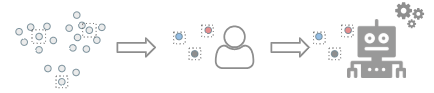
\includegraphics[width=.9\textwidth]{figures/Framework_processo_inicial.png}
  \caption{Etapa Inicial do Framework de Aprendizado Ativo}
  \label{fig:framework_AL_classico_etapa_inicial}
\end{figure}


No processo interativo já temos um classificador e um conjunto de amostras pré-rotuladas. Assim iniciamos da seguinte forma, conforme a figura ~\ref{fig:framework_AL_classico}: uma política Q seleciona um conjunto de amostras de U (1 e 2) para ser classificada por G (3). Essas amostrsas são levadas ao oráculo que aprova ou corrige a classificação de G (4). Após isso, essa amostra é incluída em T e o classificador pode ser retreinado, finalizando o ciclo (5). Esse processo pode ser repetido várias vezes até um critério de parada, como por decisão do oráculo, ou por não ter mais dados disponíveis em U, por exemplo. 


\begin{figure}
  \centering
  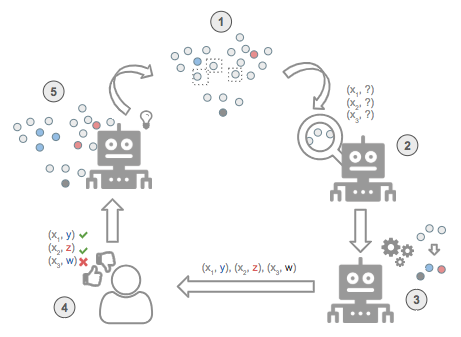
\includegraphics[width=0.9\textwidth]{figures/Framework_Active_Learning_Classico_v2.png}
  \caption{Framework Clássico de Aprendizado Ativo}
  \label{fig:framework_AL_classico}
\end{figure}


O aprendizado ativo costuma ser descrito na literatura em duas grandes etapas: i) cenários e ii) estratégia de seleção e organização das amostras [\cite{settles2014active}]. A etapa de seleção de cenários é a forma pela qual o algoritmo tem acesso aos dados. Existem diversos cenários que podem ser usados mas, independente de qual seja o escolhido, deve-se selecionar qual amostra será enviada para o oráculo através de uma função de utilidade [\cite{olsson2009literature, dasgupta2011two}]. A seguir temos a descrição detalhada dos cenários e estratégias de seleção. 


\section{Cenários do Aprendizado Ativo}
\label{sec:cenarios}

Existem alguns cenários onde o Aprendizado Ativo poderá organizar os dados para, então, fazer a seleção de queries. Dentro desses, os três principais que podem ser considerados na literatura são: (i) membership query synthesis, (ii) stream-based selective sampling e (iii) pool-based sampling \cite{settles2014active}. A figura ~\ref{fig:ActiveLearningScenarios} abaixo sintetiza a ideia.


\begin{figure}
  \centering
  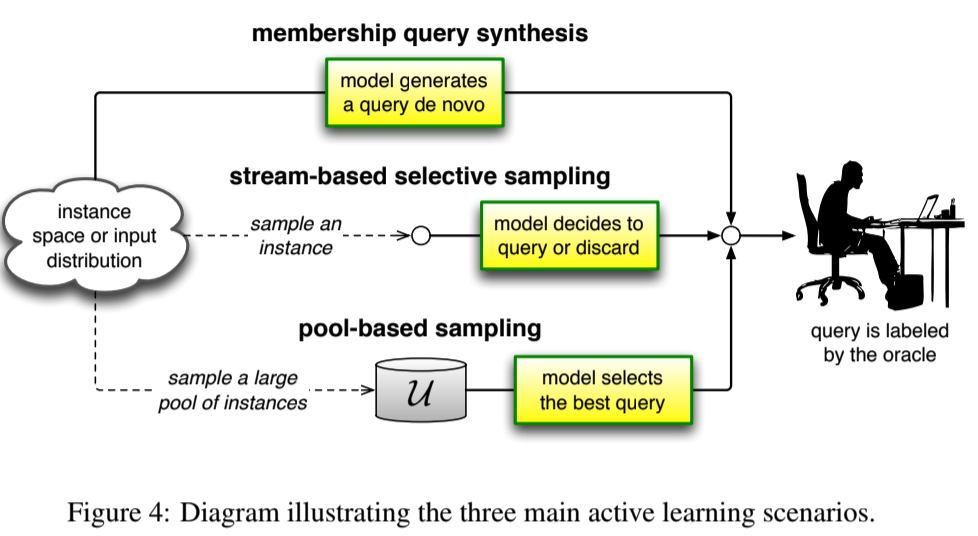
\includegraphics[width=.8\textwidth]{figures/active_learning_scenarios.png}
  \caption{Cenários de Aprendizado Ativo (Settles, 2014)}
  \label{fig:ActiveLearningScenarios}
\end{figure}


\subsection{Membership Query Synthesis}
\label{sec:cenarios_membeship}

Uma das primeiras formas de se pensar na organização dos dados foi atráves do método de membership. Neste cenário, é proposto que o algoritmo crie exemplos sintéticos para serem enviados ao oráculo. Os primeiros trabalhos que utilizaram essa ideia datam de 1980 [\cite{shapiro1981algorithm, shapiro1982algorithmic, shapiro198algorithmic_2}] e há muitas formas de se fazer isso. Podemos, por exemplo, mudar a estrutura de uma imagem ou retirar partes dela. 

De uma forma geral o que pretende-se fazer com esse cenário é, na distribuição do espaço de features, criar exemplos representativos. O trabalho de [\cite{baum1992query}] é um bom exemplo pois tentam sintetizar uma amostra através de uma rede neural de 2 camadas. O que eles prendentem, então, é encontrar, em uma dicotomia, um hiperplano que esteja entre duas amostras distintas. A figura ~\ref{fig:LangBaum_GeometryQueryLearning} do trabalho de Lang e Baum representa essa ideia. O ponto m, no meio da intersecção entre $x_+$ e $x_-$ seria uma amostra representativa.

\begin{figure}
  \centering
  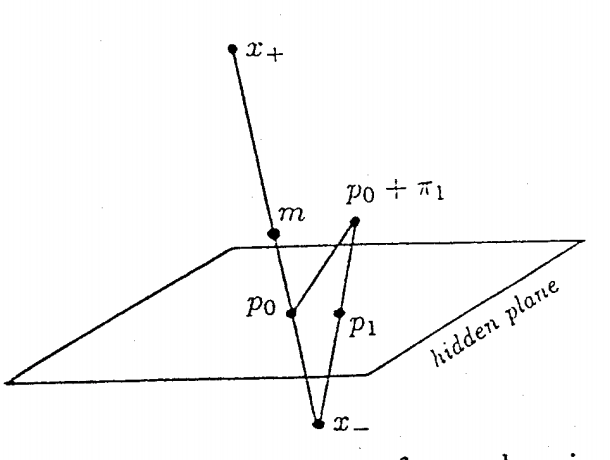
\includegraphics[width=.4\textwidth]{figures/lang_baum_geometry_query_learning.png}
  \caption{A geometria do Aprendizado por Consulta [\cite{baum1992query}]}
  \label{fig:LangBaum_GeometryQueryLearning}
\end{figure}

É importante ressaltar que há desafios nesse sentido quando temos um domínio de alta complexidade, como o caso de imagens de raio-x, por exemplo [\cite{angluin1988queries}]. Mesmo em casos que poderiam ser mais simples encontramos dificuldades. Uma das principais limitações, acontecem quando o oráculo é um humano. Na imagem ~\ref{fig:LangBaum_5vs9Example}, os autores, [\cite{baum1992query}], utilizaram da ideia acima para gerar exemplos sintéticos. O interessante é que, dependendo, de onde os pontos se enontravam, algumas imagens não possuiam nenhum significado. 

\begin{figure}
  \centering
  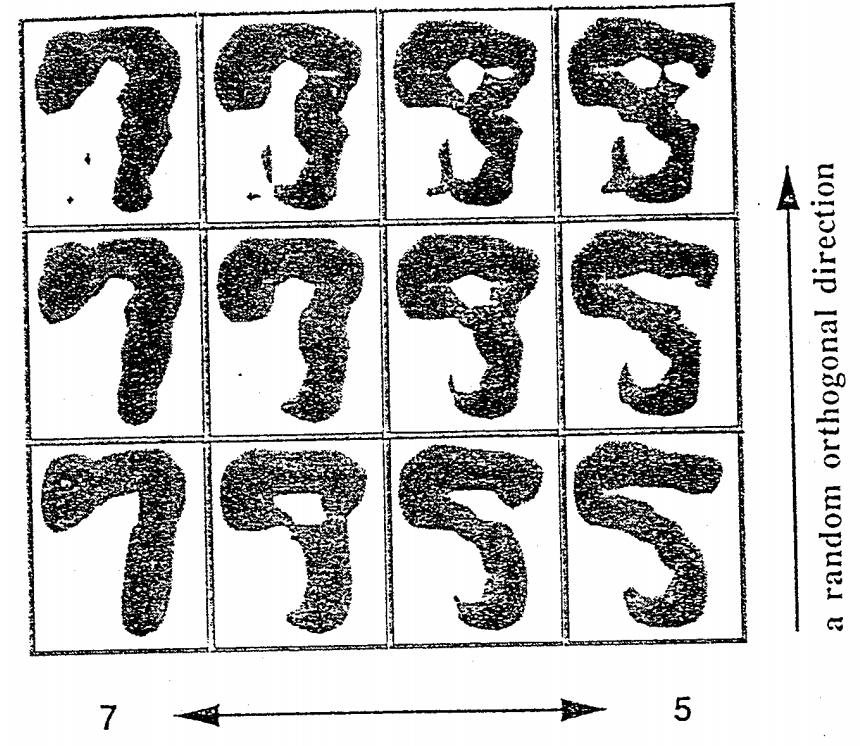
\includegraphics[width=.4\textwidth]{figures/lang_baum_5_vs_9_example.png}
  \caption{Exemplos Sintéticos sem Significado [\cite{baum1992query}]}
  \label{fig:LangBaum_5vs9Example}
\end{figure}

Apesar dessa limitação para oráculos humanos, o trabalho [\cite{king2004functional, king2009automation}] conseguiu utilizar eficientemente essa ideia para quando o oráculo é um robo. Além desse, há um trabalho que utilizou de Genrative Adversarial Networks (GAN) em conjunto com Aprendizado Ativo para criar exemplos [\cite{zhu2017generative}]. O interessante é que eles revisitaram o trabalho de Lang e Baum e conseguiram criar exemplos significativos no caso de digitos, conforme a figura ~\ref{fig:GAN_5_vs_9}. Entretanto, geraram amostras sem significado para fotos de caes e gatos. 

\begin{figure}
  \centering
  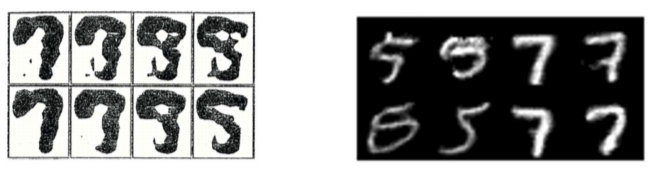
\includegraphics[width=.9\textwidth]{figures/generative_GAN_AL_5_vs_9.png}
  \caption{Esquerda: exemplo de \cite{baum1992query} revisitado e na foto à direita o exemplo gerado pela GAN. [\cite{zhu2017generative}]}
  \label{fig:GAN_5_vs_9}
\end{figure}


Há, ainda, outras iniciativas com esse cenário. No trabalho de [\cite{wang2015active}], por exemplo, utiliza-se o paradigma de criar exemplos sintéticos mas, ao final, utilizar exemplos da própria base de dados para serem enviados ao oráculo. A ideia é parecida com o que foi citado acima mas, ao invés de criar amostras, a proposta é de utilizar a posição deles e utilizar dos vizinhos, pois eles serão reconhecidos por um humano e tem grande chance de serem informativos. A figura ~\ref{fig:wang_2015_membership}  mostra essa ideia. 

\begin{figure}
  \centering
  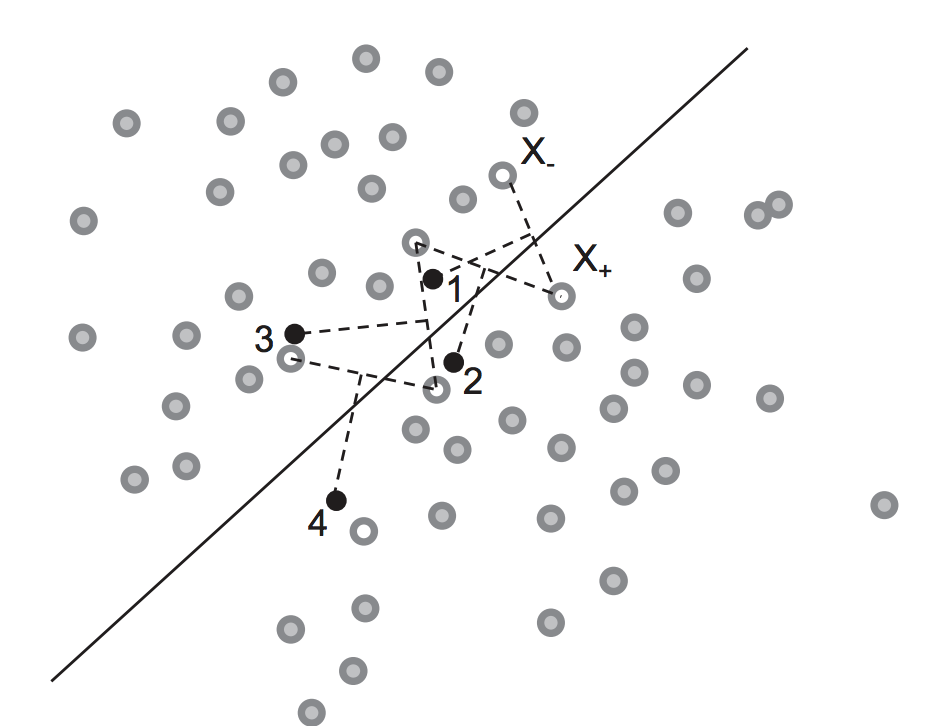
\includegraphics[width=.5\textwidth]{figures/wang_2015_membership.png}
  \caption{Exemplos representativos a partir da posição de amostras sintéticas [\cite{wang2015active}].}
  \label{fig:wang_2015_membership}
\end{figure}


\subsection{Stream-based Selective Sampling}
\label{sec:cenarios_selective_sampling}

Neste cenário permanece a premissa de que temos muitas amostras sem rótulos. No entanto, elas são sequencialmente escolhidas e, então, selecionadas por algum critério quantitativo para, assim, serem levadas ao oráculo. Quando as amostras são escolhidas não se sabe ainda se ela será selecionada. É através de alguma medida de incerteza, que será discutida nas próximas seções, que essa amostra será levada ao oráculo ou descartada. É interessante notar que se a distribuição dos dados for uniforme, não teremos qualquer vantagem sobre o cenário anterior. Entretanto, se for não-uniforme e desconhecida, saberemos que as consultas serão sensíveis a esse fato [\cite{settles2014active}]. A figura ~\ref{fig:settles_2014_selective_sampling} mostra o fluxo. 

Há algumas situações específicas pelas quais é interessante utilizar o cenário sequencial de amostras. A mais comum é quando temos, por exemplo, uma limitação no poder computacional ou de memória. Nesses casos torna-se inviável processar o conjunto de dados sem rotulação de uma única vez. Outro exemplo interessante é quando temos aplicações na web. Nesses casos, também chamado de Online Learning, é interessante que as amostras sejam escolhidas de maneira sequencial. O trabalho de [\cite{chu2011unbiased}], motivado pelos milhões de dados diários do Yahoo, mostra como esse cenário pode ser benéfico. 


\begin{figure}
  \centering
  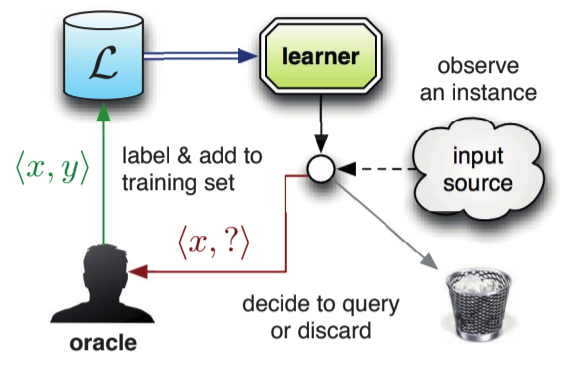
\includegraphics[width=.5\textwidth]{figures/settles_2014_selective_sampling.png}
  \caption{Fluxo do cenário de Selective Sampling [\cite{settles2014active}].}
  \label{fig:settles_2014_selective_sampling}
\end{figure}

\subsection{Pool-based Sampling}
\label{sec:cenarios_pool}

Dos três cenários conhecidos na literatura, o pool-based é o mais utilizado em casos reais, enquantos os anteriores são mais comuns em trabalhos teóricos. Diferentemente do cenário de selective sampling, onde uma das motivações era a falta de recursos, como poder computacional ou memória, aqui escolhemos, de inicio, todo o conjunto de dados. Assume-se, neste caso, que tenhamos um conjunto muito grande de dados sem rótulos e um pequeno conjunto de amostras rotuladas. Também temos que esse conjunto seja estático, embora isso não seja estritamente necessário. A maior diferença entre os dois é que enquanto o primeiro escolhe as amostras sequencialmente e, então, decide, o pool analisa todas as amostras e, através de uma medida de utilidade, seleciona [\cite{settles2014active}]. A imagem ~\ref{fig:settles_2014_pool}  demostra o fluxo.

\begin{figure}
  \centering
  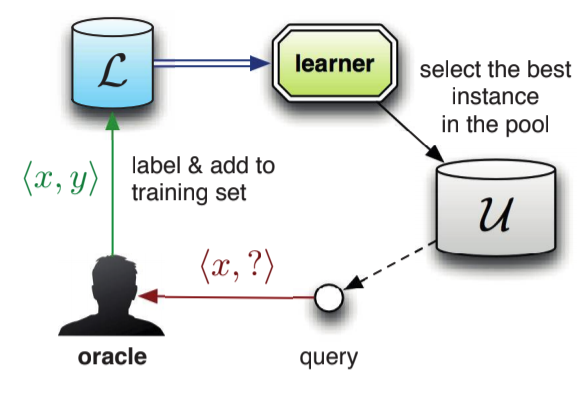
\includegraphics[width=.5\textwidth]{figures/settles_2014_pool.png}
  \caption{Fluxo do cenário de Pool-Based Sampling [\cite{settles2014active}].}
  \label{fig:settles_2014_pool}
\end{figure}

%Existem muitos trabalhos recentes que utilizam esse cenário. Por exemplo: \todo{citar trabalhos}



\section{Estratégia de Seleção e Organização das Amostras}
\label{sec:query_strategy}

Todos os cenários de Aprendizado Ative discutidos anteriormente envolvem avaliar a representatividade das amostras a serem escolhidas. Há muitas formas propostas de se fazer isso na literatura e, a seguir, temos as principais delas [\cite{settles2012active}]. É importante notar que em todas as estratégias teremos alguma medida quantificável para selecionar as amostras. Por vezes podemos ter estratégias diferentes que utilizam medidas iguais ou similares.




\subsection{Amostras Incertas} %uncertainty sampling 
\label{sec:amostras_incertas}

Amostras Incertas é uma das estratégias mais utilizadas em Aprendizado Ativo. Isso acontece provavelmente por ser muito intuitiva e de fácil implementação [\cite{settles2014active}]. A ideia básica é que precisamos encontrar exemplos que, por terem um alto grau de incerteza, serão os mais representativos. Ou seja, queremos descartar exemplos onde o classificador já possui uma alta probabilidade de acerto e focar nos exemplos mais incertos.  


\begin{figure}
  \centering
  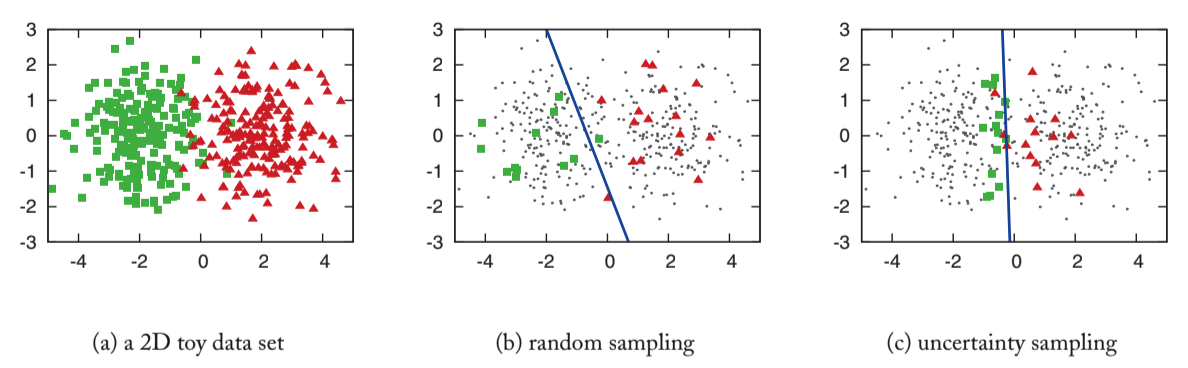
\includegraphics[width=1.0\textwidth]{figures/settles_2014_uncertainty_sampling_example.png}
  \caption{Exemplo de Amostras Incertas [\cite{settles2014active}].}
  \label{fig:settles_2014_uncertainty_example}
\end{figure}

A figura ~\ref{fig:settles_2014_uncertainty_example} exemplifica bem a ideia exposta. Nela temos como classificador uma regressão logisitca treinada em (b) por 30 amostras aleatórias e em (c) por 30 amostras mais representativas. É perceptível, comparando com (a), que o classificador pelas amostras incertas está muito acertivo. Isso ocorre porque as amostras mais representativas estarão, nesse caso, próximas da linha vertical que separa os dois grupos de dados.

Apesar da ideia ser intuitiva precisamos encontrar uma forma de medir a incerteza das amostras. É importante notar que uma interpretação probabilística pode ajudar. Isso porque, quando colocamos nesse escopo, conseguimos generalizar e modelar essa ideia para uma enorme de casos. Sendo o $x^*_{A}$ a melhor consulta possível utilizando a medida $A$, podemos pontuar as três principais formas de medir a incerteza de uma amostra [\cite{settles2014active}]:

\textbf{Menos Confiante:} nessa medida estamos interessados nos exemplos que são mais prováveis de serem classificados de forma errada. Uma maneira de formular isso seria:

\begin{align*}
\textbf{X}^*_{LC} = &\arg\min_{x} P_{\theta}  (\hat{y}\lvert x)\\
&\arg\max_{x} 1 - P_{\theta}  (\hat{y}\lvert x)\\
\end{align*}

\textbf{Margem:} similar a medida anterior, a margem utiliza da primeira e segunda maiores probabilidades de uma determinada classe. Intuitivamente, caso a margem fique muito alta, significa que o classificador não possui uma incerteza muito grande em relação à classe adotada. Ao contrário, caso a margem fique estreita, o calssificador não sabe ao certo a qual classe aquela amostra pertecen:

\begin{align*}
\textbf{X}^*_{M} = &\arg\min_{x}[ P_{\theta} (\hat{y_{1}}\lvert x) - P_{\theta} (\hat{y_{2}}\lvert x)]\\
&\arg\max_{x}[ P_{\theta} (\hat{y_{2}}\lvert x) - P_{\theta} (\hat{y_{1}}\lvert x)]\\
\end{align*}

\textbf{Entropia:} leva em consideração todas as probabilidades que uma amostra pode ser classificada. Nesse sentido, a entropia pode ser entendida como uma medida de impureza. 

\begin{align*}
\textbf{X}^*_{H} = &\arg\max_{x} H_{\theta}  (Y\lvert x)\\
&\arg\max_{x} \sum_{y} P_{\theta}  (y\lvert x) \log_{} P_{\theta}  (y\lvert x)\\
\end{align*}





\begin{figure}
  \centering
  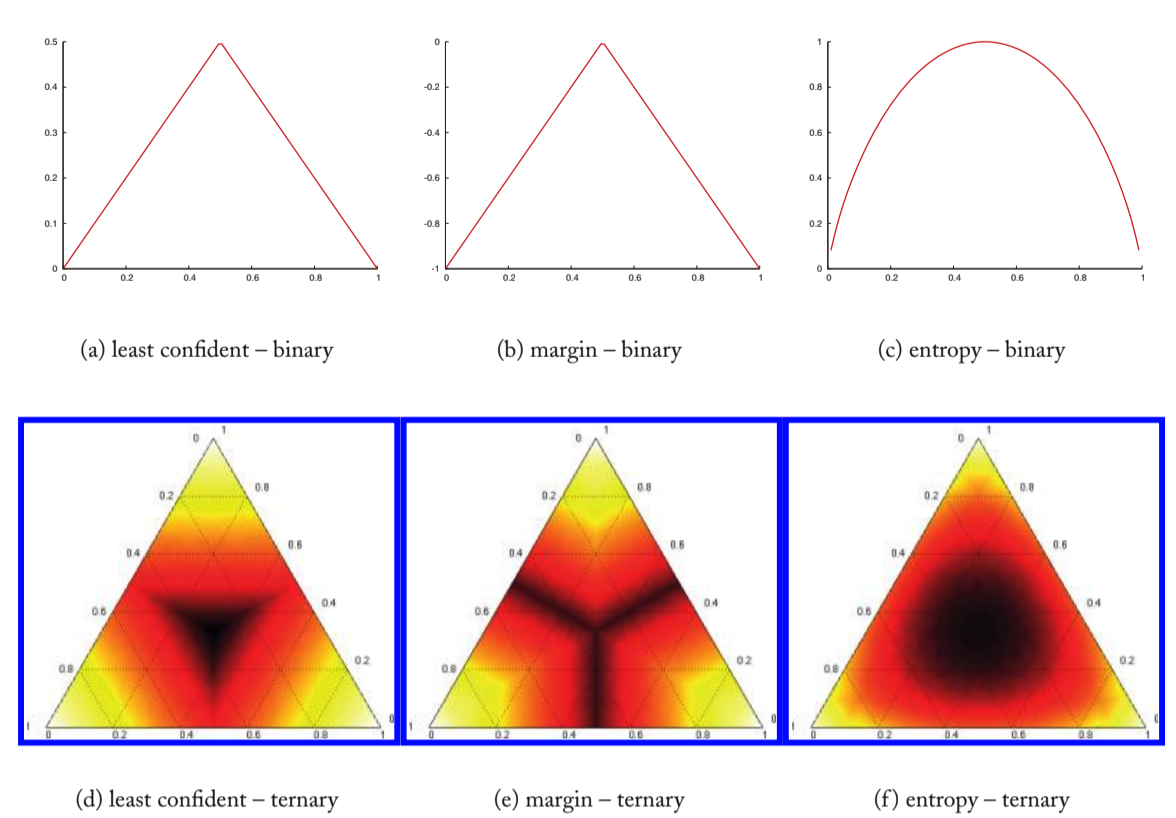
\includegraphics[width=0.9\textwidth]{figures/settles_2014_uncertainty_medidas.png}
  \caption{Comparação entre as três medidas [\cite{settles2014active}].}
  \label{fig:settles_2014_uncertainty_medidas}
\end{figure}



Das três medidas acima, é importante notar que a primeira leva em consideração apenas a maior probabilidade, enquanto a segunda apenas as duas maiores. A última, por outro lado, considera todas as possíveis classificações de uma amostra. Por isso mesmo é a mais comumente utilizada [\cite{settles2014active}]. Uma forma forma de comparar as três medidas pode ser vista na figura ~\ref{fig:settles_2014_uncertainty_medidas} abaixo. Nela é possível ver o resultado das funções de utilidade como função da probabilidade de determinada classificação. Assim, percebemos em um exemplo dicôtomico, na parte superior, que sempre que a probabilidade da classificação for 0.5, teremos o maior resultado de utilidade daquela medida. Da mesma forma, na parte inferior, em um exemplo com três possíveis classificações, percebemos a mesma coisa. 


\subsection{Espaço de Hipóteses} 
\label{sec:hypothesis_space}

Uma outra estratégia que pode ser utilizada é procurar amostras dentro do espaço de hipóteses [\cite{mitchell1978version, mitchell1982generalization}. Nessa estratégia trabalharemos, por exemplo, com mais de um classificador ou com configurações diferentes de um mesmo classificador. Essa ideia foi implementada no trabalho de [\cite{atlas1990training,cohn1994improving}\ e pode ser vista na figura ~\ref{fig:cohn_1994_hypothesis_space_example}. Nela temos dois tipos de classificações (0 ou 1) e quatro hipóteses diferentes. As áreas mais escuras, onde há a interseção das diferentes hipóteses, representam a região onde pode-se haver as amostras mais incertas. 

\begin{figure}
  \centering
  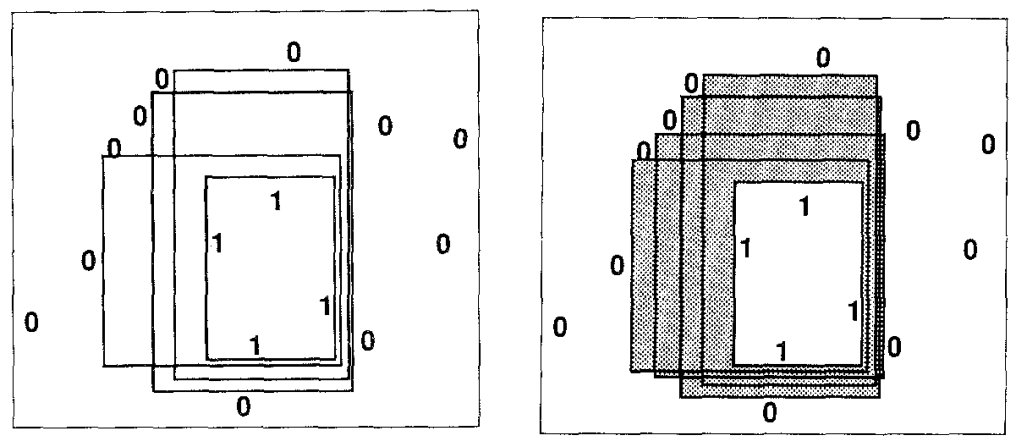
\includegraphics[width=0.8\textwidth]{figures/cohn_1994_hypothesis_space_example.png}
  \caption{Exemplo Espaço de Hipóteses [\cite{cohn1994improving}].}
  \label{fig:cohn_1994_hypothesis_space_example}
\end{figure}

Um exemplo mais canônico pode ser visto no trabalho de [\cite{dasgupta2011two}], onde temos quatro classificadores lineares e a região em rosa representa a área de incerteza. Nessa estratégia uma amostra só iria ser selecionada se estivesse nessa região.

\begin{figure}
  \centering
  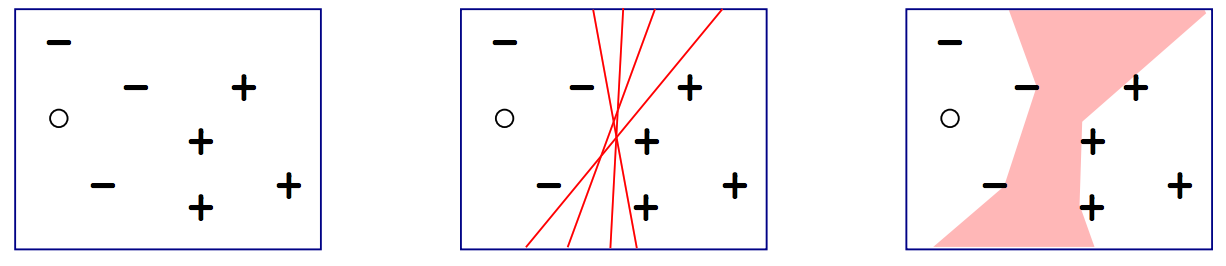
\includegraphics[width=0.9\textwidth]{figures/dasgupta_two_faces_hypothesis_example.png}
  \caption{Exemplo Espaço de Hipóteses [\cite{dasgupta2011two}].}
  \label{fig:dasgupta_two_faces_hypothesis_example}
\end{figure}

É importante pontuar que, como mostrado no trabalho de [\cite{settles2014active}], a ideia de procurar no espaço de hipóteses possui duas frentes principais: (i) consultas por desacordo e (ii) consultas por comite [\cite{seung1992query}]. As duas utilizam o mesmo paradigma que é de reduzir o espaço de hipóteses, mas consideram premissas diferentes. O trabalho de [\cite{cohn1994improving}], por exemplo, utiliza de uma aproximação, onde temos duas redes neurais que estão nos extremos do espaço de hipóteses e quando há um desacordo entre as classificações encontramos uma região de interesse. Apesar de ambas serem muito similares, elas possuem premissas diferentes. No primeiro, por exemplo, temos que a noção de desacordo necessita ser mensurada em todo o espaço de hipóteses, ou pelo menos em extremos, e precisa ser uma mensuração binária. A consulta por comite, por outro lado, relaxa um pouco essas premissas. De qualquer forma, nos últimos anos, entende-se que todo paradigma que utiliza um comitê ou conjunto, $C =$ { $\theta^{(1)}$, ..., $\theta^{(C)}$}, de hipóteses é considerado como consulta por comitê [\cite{settles2012active, settles2014active}].


Assim como ocorre na estratégia anterior, é necessário que tenhamos como medir a incerteza entre as diversas hipóteses. Há, na literatura, duas formas principais de se fazer isso: 

\textbf{Entropia por Voto:} a abordagem sugerida por [\cite{dagan1995committee}] considera todas as possíveis classificações e o número de votos que receberam. 

\begin{align*}
\textbf{X}^*_{SVE} = &\arg\max_{x} \sum_{y} P_{C}  (y\lvert x) \log_{} P_{C}  (y\lvert x)\\
\end{align*}

\textbf{Divergência de Kullback-Leibler (KL):} a abordagem sugerida por [\cite{mccallumzy1998employing}] utiliza de uma abordagem probabiblistica, vinda da divergência de KL.

\begin{align*}
\textbf{X}^*_{KL} = &\arg\max_{x} \sum_{\theta} KL(  P_{\theta} (Y\lvert x) \lvert\lvert P_{C} (Y\lvert x))\\
\end{align*}


\subsection{Amostras Incertas vs. Espaço de Hipóteses} 
\label{sec:minimizing_expected}

Uma das limitações das Amostras Incertas ocorrem no fato de que, como temos poucos dados, é possível que tenhamos um processo de aprendizado míope, principalmente porque não olhamos para todos os exemplos [\cite{settles2014active}]. A parte superior da figura ~\ref{fig:limitations_incertas} ajuda a exemplificar esse problema. Nesse caso, por não termos dados suficientes, o algoritmo falhou em trazer dados que estão no meio dos triângulos. Com isso, tivemos um output extremamente diferente do que o esperado. Esse tipo de caso não é comum, mas ocorre de resultarem em piores resultados do que se fossem amostras randômicas. A parte inferior da figura mostra a estratégia do Espaço de Hipóteses para o mesmo caso. É possível ver que os resultados são muito melhores. 


\begin{figure}
  \centering
  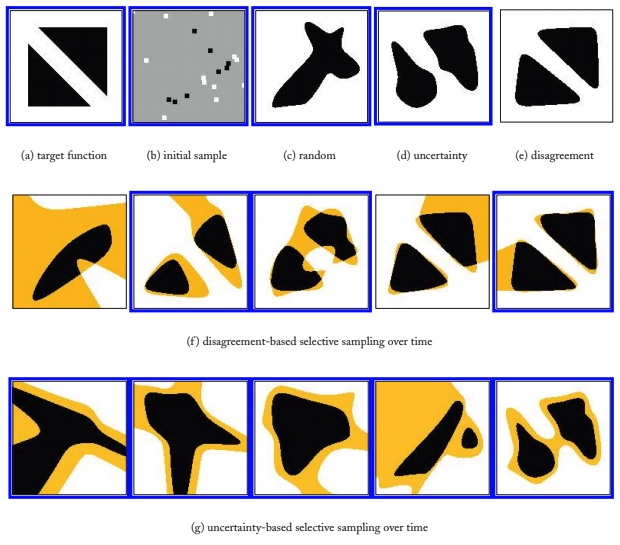
\includegraphics[width=0.8\textwidth]{figures/limitations_incertas.png}
  \caption{Limitações Amostras Incertas [\cite{settles2014active}].}
  \label{fig:limitations_incertas}
\end{figure}

Uma outra limitação, tanto das Amostras Incertas quanto no Espaço de Hipóteses, ocorre no fato de que elas são muito suscetíveis a outliers. Isso ocorre porque, nas duas estratégias, as amostras são medidas individualmente [\cite{settles2014active}]. Ou seja, não é levado em consideração a distribuição delas. A figura ~\ref{fig:limitations_outliers} ajuda a sintetizar esse caso. Nela o exemplo A seria o escolhido pois está exatamente na linha de divisão entre as duas classes. Entretanto, por ser um outlier, não é um exemplo realmente representativo. 


\begin{figure}
  \centering
  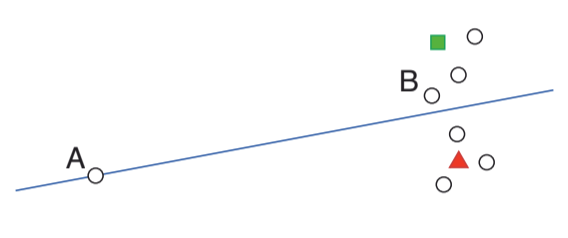
\includegraphics[width=0.5\textwidth]{figures/limitations_outliers.png}
  \caption{Limitações com Outliers [\cite{settles2014active}].}
  \label{fig:limitations_outliers}
\end{figure}

 \subsection{Explorando a Estrutura dos Dados} 
\label{sec:explorando_estrutura_dados }

Uma das maneiras encontradas para resolver a limitação dos outliers é explorar a estrutura dos dados. Uma das formais interessantes de se fazer isso é utilizando a intersecção do Aprendizado Ativo com o Aprendizado Semi-Supervisionado. Podemos, por exemplo, utilizar a estrutura dos dados e encontrar clusters através de alguma medida de similaridade [\cite{saito2014active, dasgupta2011two}]. Selecionamos algumas amostras, como os centroides ou o mais informativos, e pedimos para o oráculo categorizar corretamente, iniciando, assim, o ciclo do aprendizado ativo. 

Há, porém, alguns problemas na estratégia. Não temos um número óbvio de clusters. Também podemos ter vários níveis de granularidade e, o pior dos casos, os clusters podem não representar as categorias corretas do dataset [\cite{dasgupta2011two, settles2014active}].  A figura XXX mostra bem essa ideia \todo{criar toy example}.

\section{Aprendizado Ativo com Participação Ativa do Usuário}
\label{sec:aprendizado_ativo_variacoes}

O aprendizado ativo tem como principal objetivo diminuir o esforço gasto na rotulação de amostras tendo, como resultado, um bom classificador. Há outras técnicas que são correlatas a essa ideia, como o aprendizado semi-supervisionado [\cite{zhu2006semi}], que utiliza da própria estrutura dos dados para re-treinar o classificador. Outra técnica interessante é o transfer learning, que tem como objetivo passar um conhecimento prévio de um problema já resolvido para algum outro similar [\todo{colocar referencias}]. Além desses que foram citados podem existir diversas variações [\todo{colocar referencias}]. A diferença básica é que no aprendizado ativo temos a interação de um oráculo, sendo na maioria das vezes um humano. 


Apesar dessa ideia ser muito interessante, principalmente quando temos um domínio que requer profissionais extremamente especializados para categorizar as amostras, o oráculo ainda é utilizado de forma muito limitada no framework clássico [\cite{seifert2010user}]. Nele sua utilização se restringe em aceitar/corrigir as classes dadas pelo classificador. Há uma ideia em tentar dar ao oráculo outros papéis. Na realidade, existe um grande interesse em como incorporar mais conhecimento humano dentro dessa estrutura [\cite{settles2014active}]. 

O trabalho de [\cite{castro2009human}] foi um dos primeiros a tentar relacionar, de forma quantitativa, o aprendizado ativo com a ciência cognitiva. Nesse caso o problema era conseguir identificar duas classes de ovos alienígenas que se diferenciavam pela forma. Enquanto o primeiro grupo poderia poderia escolher quais ovos teriamn  informações a respeito, o segundo apenas recebia as imagens com a respectiva classe. O estudo mostrou que os resultados foram melhores para o grupo que pôde escolher ativamente as amostras. Um estudo parecido foi feito por [\cite{markant2014better}] e, para determinados casos, confirmou esse cenário. 

O interesse em unir o conhecimento humano, incorporando-o no loop de aprendizado, continua em aberto. Um estudo recente [\cite{kottke2018other}] teve como objetivo mudar a posição do humano de ser um especialista em categorizar amostras para ser também um especialista em selecionar. No estudo foi possível demonstrar resultados positivos, onde o aprendizado computacional pode se beneficiar com a interação humana. Outros estudos [\cite{calma2016active}] mostram que esse é um desafio atual. Inclusive, há uma linha de pesquisa interessante que pretende fazer isso com o apoio de análises visuais, como a utilização de grafos e projeções em 2D [\cite{yang2018visually, bernard2018comparing, weigl2016mapview}].

%% comentar aqui o rtablaho do settles com NLP

%% falar quer e exclusivamente nos casos onde termos a necessidade de um especialista. Lembrar do trabalho do Baum que nao deu certo (exemplos sinteticos que nao faizam nenhum sentudo!)